
\textit{}\chapter{Stávající metody a aplikace}
Tato kapitola pojednává o aktuálně používaných metodách v rozpoznávání v obraze. Jsou zde rozberány aplikace, které kameru Kinect již využívání i potenciální použití v dalších oborech.

\section{Stávající metody zpracování obrazu}
Cílem této kapitoly je rešerše akutálních metod rozpoznávání lidí, těla a jeho částí. Nezbytnou součástí je i tomu předcházející úprava načteného obrazu. Berou se zde v potaz stávající metody, které mohou sloužit k účelům této práce.

Předzpracování obrazu se týká všech aplikací využívajícíh digitální obrazy z kamery. Při zpracování digitálních obrazů je potřeba obraz rozostřit kvůli odstranění extrémů z obrazu, následně jsou probírány již věci specificky pro zpracování obrazu k detekci objektů.

\subsection{Rozostření}
Rozostření slouží k eliminaci šumu v obraze. Nejosvědčenější metody jsou nízkofrekvenční filtry jako je Gauss a medián. Tato kapitola čerpá ze závěrečné práce Pikory~\cite{15}, přesněji kapitoly 5 a 6.\\

Filtr medián se zaměřuje na vyhlazování lokálních extrémů v obraze. Nezachovává jemné čáry a ostré rohy, takže je vhodný pouze v aplikacích, kde na tom nezáleží. Výraznou výhodu představuje v odstranění extrémů, které v obraze mohou vzniknout. Narozdíl od průměrování není obraz zkreslený kvůli chybným pixelům, které mají výrazně odlišnou hodnotu.
 
Velikost okolí zahrnutého v analýze lze zvětšit při větší hustotě šumu. Pokud v aplikacích záleží na hranách, je důležité zachovat určité rozlišení. Na obrázku~\ref{pic1} lze pozorovat rozdíly mezi filtrem s průměrováním (b) a filtrem s mediánem (c).\\

\begin{figure}[h]
\centering
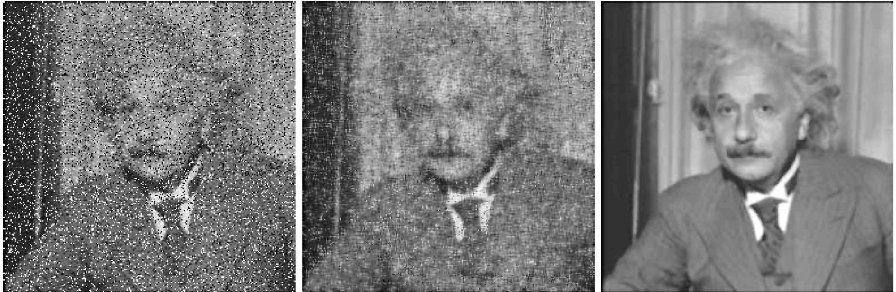
\includegraphics[width=0.8\linewidth]{median.jpg}
\caption{a) původní obraz b) průměrování c) medián\\
 (Převzato z ~\cite{15}) }
 \label{pic1}
\end{figure}

\newpage
Gaussovský filtr je průměrování s Gaussovským rozložením. Využívá se k vyhlazování obrazu, odstranění detailů a šumu. Obrázek~\ref{pic2} zachycuje rozdíl mezi opakovanou aplikací Gaussovského filtru. Výpočet hodnoty pro každý pixel je uveden ve vzorci:
\begin{eqnarray}
G(x,y) = \frac{1}{2 \pi \sigma^{2}}*e^{-\frac{x^{2}+y^{2}}{2\sigma^{2}}}  ,
%ae^{-\frac{(x-b)^{2}}{2c^{2}}}
\label{gauss}
\end{eqnarray}
kde $ x $ a $ y $ jsou souřadnice daného pixelu a $ \sigma $ je směrodatná odchylka.\\

V konvoluční masce se přidělí větší váha bodu ve středu, aby se zabránilo rozšíření rozostření do nekonečna. Aby se aplikací konvoluční masky neměnila světlost, součet všech složek konvoluční matice dává hodnotu 1. Příklad konvoluční masky:
\begin{eqnarray}
\frac{1}{16} \begin{bmatrix}
1 & 2 & 1 \\
2 & 4 & 2 \\
1 & 2 & 1
\end{bmatrix}
\end{eqnarray} 

\begin{figure}[h]
\centering
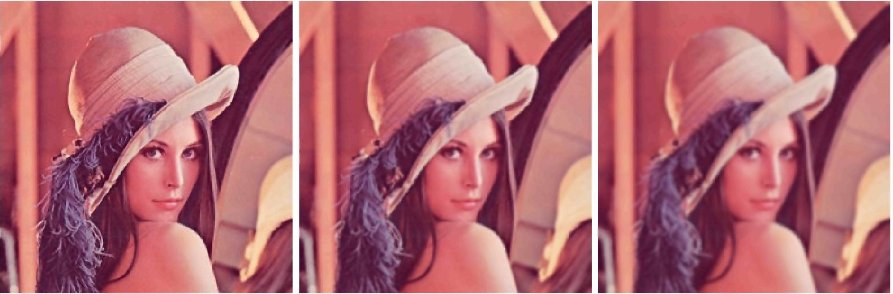
\includegraphics[width=0.8\linewidth]{gauss.jpg}
\caption{a) původní obraz b) jednou aplikovaný Gaussovský filtr c) třikrát aplikovaný Gaussovský filtr. (Převzato z ~\cite{15}) }
\label{pic2}
\end{figure}

\subsection{Prahování}
Většina metod se zakládá na zpracování binárního obrazu. Princip je ve zvolení prahové hodnoty, se kterou se všechny hodnoty porovnají. Pokud hodnota přidělená (v případě RGB kamery) nebo načtená (v případě hloubkové kamery) větší než prahová, do výsledného obrazu se uloží '1', v opačném případě se zapíše '0'. Objekt, který je středem zájmu, se skládá z pixelů s hodnotou 1 zatímco ostatní mají hodnotu 0. Metoda prahování (anglicky tresholding) se dělí na více druhů: lokální, pásmové, polo-prahování, multi-prahování a další.~\cite{hlav}

\subsection{Nalezení kostry}
Při hledání topologie a tvaru objektu lze použít například skeletonizaci. Ve zjednodušené představě se jedná o zredukovaný objekt, který představuje minimální dostačující reprezentaci zkoumaného objektu, která obsahuje všechny významné body. Tato kapitola vychází z Palagyiova přehledu~\cite{25}. Existují tři způsoby hledání kostry:

\begin{itemize}
\item detekce ze vzdálenostní mapy,
\item výpočet Voronoiova diagramu, který je generován pomocí hraničních bodů a
\item ztenčení.
\end{itemize}

Jelikož nelze zaručit, že se jedná o přesnou kostru objektu, jsou zde dva rozhodovací faktory. Jedná se o požadavek zachování topologie a geometrickou podmínku, která vynucuje umístění kostry do středu objektu. Topologickou podmínku splňuje Voroného diagram a ztenčování, geometrickou zaručuje detekce ze vzdálenostní mapy a Voroného diagram.

Detekce ze vzdálenostní mapy lze popsat třemi kroky. Nejdříve se v binárním obraze označí hraniční body objektu (zelené pixely na obrázku~\ref{distance}). Poté se vygeneruje vzdálenostní mapa podle toho, jak daleko se nachází konkrétní pixel od nejbližšího hraničního bodu. Hrany kostry reprezentují pixely, které jsou lokálními extrémy ve výsledné vzdálenostní mapě.
\begin{figure}[h]
\centering
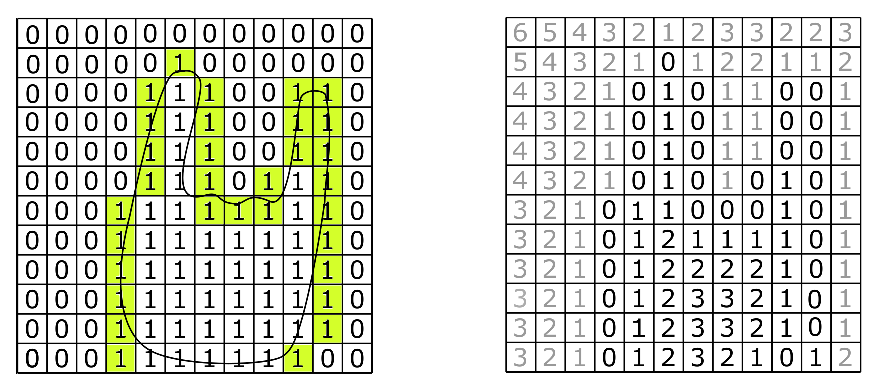
\includegraphics[width=0.8\linewidth]{distance.eps}
\caption{Zelené pixely na levém obrázku označují hranice zpracovávaného objektu. Vůči nim se vypočítává vzdálenost zbylých pixelů, z nichž lokální maxima představují kostru. Výpočet probíhá pomocí čtyř sousedních pixelů. (Vlastní zpracování.)}
\label{distance}
\end{figure}

Voroného diagramy dělí prostor na části podle množiny bodů tak, aby se v každé oblasti nacházel právě jeden bod. Do množiny bodů se přidá část hraničních bodů objektu (červené body na obrázku~\ref{picVoi}). Sousedící okraje nalezených částí tvoří kostru. Čím více bodů množina obsahuje, tím přesnější kostra bude.
\begin{figure}[h]
\centering
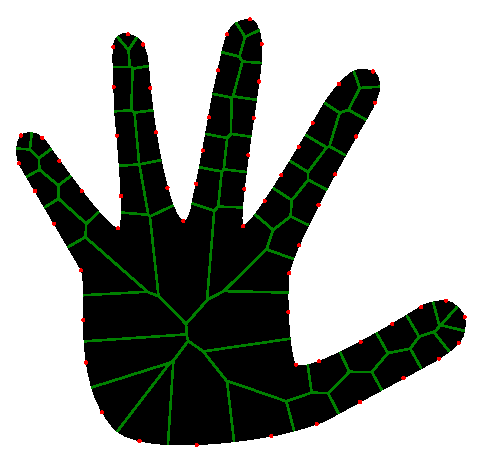
\includegraphics[width=0.4\linewidth]{hand_voi.eps}
\caption{Červené body reprezentují zvolené body na kraji ruky. Zelené čáry zobrazují hranice sousedících oblastí. (Vlastní zpracování.)}
\label{picVoi}
\end{figure}

Ztenčování je proces, který se opakuje tak dlouho, dokud se v obraze vyskytují pixely, jejichž odstranění neporušuje předem definované podmínky a tudíž se výsledná kostra stále ztenčuje a zároveň zůstává zachována topologická podmínka. Podmínky se mohou lišit podle toho, k jakým účelům je algoritmus používán.

\subsection{Detekce hran}
K rozpoznávání v obraze lze dobře využít nalezených hran. Za hrany lze považovat místa, ve kterých se výrazně mění jas. K výpočtu hran se používá gradient, což je vektorová veličina určující směr a strmost největšího růstu funkce~\cite{hlav}.

Mezi vysokofrekvenční filtry, které se používají na zpracování digitálního obrazu, patří i Laplaceův filtr. Ve výpočtu se užívá gradient. Laplaceův filtr využívá pouze velikost gradientu a pro její odhad se používá všesměrový operátor vycházející z parciálních derivací. Nevýhodou je, že některé hrany detekuje dvakrát.  Vzorec pro výpočet hodnoty pixelu je:

\begin{eqnarray}
\nabla^{2}g(x,y) = \frac{\delta^{2}g(x,y)}{\delta x^{2}} + \frac{\delta^{2}g(x,y)}{\delta y^{2}}.
\end{eqnarray} 
Laplacián je aproximován diskrétní konvolucí. Příklad konvolučního jádra může být:
\begin{eqnarray}
\begin{bmatrix}
0 & 1 & 0 \\
1 & -4 & 1 \\
0 & 1 & 0
\end{bmatrix}.
\end{eqnarray} 

\section{Rozpoznávání v obraze}
\label{rozpoznavani}
\subsection{Rozpoznávání postav}
Mezi hlavní možnosti přístupů k implementaci detekce postav z obrazu patří:
\begin{itemize}
\item na základě modelu,
\item strojově naučené programy,
\item neuronové sítě, nebo %-radial basis funkction
\item transformační matice vzdálenostní mapy ~\cite{Cham}.\\
\end{itemize}

Jednou z metod je dle Ch. Nakajima a spol.~\cite{6} ukládání několika obrázků, z nichž se detekuje pohybující se objekt a vše, co se nehýbe, se označí jako pozadí a ignoruje. Následně se naleznou kraje možné postavy, aby se vylepšil výsledek a vymazal šum. Pokud se jedinec pohybuje v druhém kroce, oříznutí probíhá z posledního získaného obrazu. Pokud nebyl detekován žádný jedinec, tak se do paměti uloží pozadí, které se z následujících obrazů rovnou vymaže pro větší přesnost. K vlastní identifikaci se používá SVM (support vector machines) a k-NN klasifikátor.\\

Hussein a spol.~\cite{9} rozpoznávají postavy tím, že prohledají obraz a porovnají siluety s databází, ve které jsou vzory lidských postav ve formě binárního obrazu. Shoda je detekována pomocí zkosení objektů. Vzdálenost D mezi vzorem V a objektem z obrazu O se počítá vzorcem
\begin{eqnarray}
 D(O,V) = \frac{1}{|V|}\sum_{i}^{}C_{i}V_{i}   ,
\end{eqnarray}

kde |V| je počet pixelů v siluetě ve vzoru, $ T_{i} $ je hodnota pixelu $ i $ ve vzoru a $ C_{i} $ je rozdíl zkosení pixelu $ i $ v obraze. Čím menší hodnota mezi vzorem a obrazem, tím lepší shoda je detekována.
%// (patří do nového odstavce?)

Nalezení podobnosti zkosením předpokládá již nalezené hrany objektů v obraze. Vzor se překryje s objektem a transformací bodů jednoho objektu pomocí parametrických transformačních rovnic.\\

Jiný přístup nalézá objekt v zorném poli pomocí hloubkové kamery. Následuje rozhodnutí, zda má objekt lidské nohy nebo alespoň dva objekty odpovídající jejich tvaru, pokud ano, tak se přejde k dalšímu kroku, ve kterém se detekuje barva kůže z RGB vstupu. Nalezený výsledek slouží jako oblast k detekci obličeje, čímž je nalezen člověk~\cite{10}.\\

Gavrila ~\cite{7} se snaží snížit výpočetní náročnost tak, že nahrazuje procházení obrazu postupně schopností se zaměřit na jeden úryvek přímo a ve druhém kroce teprve hledá podobnosti tvarů. Dosahuje tak zpracování bez časové prodlevy.
%These pixel values form a distribution of distances of the template features to the nearest features in the image
Shodu podle tvaru detekuje pomocí vzdálenosti křivek, která se počítá podobně jako u Hussein a spol.~\cite{9} podle vzorce: 

\begin{eqnarray}
 D(O,V) = \frac{1}{|V|}\sum_{t\in T}^{}d_{I}(t) ,
\end{eqnarray}
kde |V| je počet prvků ve vzoru a $ d_{I}(t) $ představuje vzdálenost daného prvku ve vzoru a jemu odpovídajícímu v obraze. Pokud je výsledná hodnota menší než předem určená prahová hodnota, považuje se objekt v obraze za postavu. Detekce chodce podle vzoru lze pozorovat na obrázku~\ref{pic3}. \\
%hlubší pozornost na předposlední odstavec na str. 4 !!!!
\begin{figure}[h]
\centering
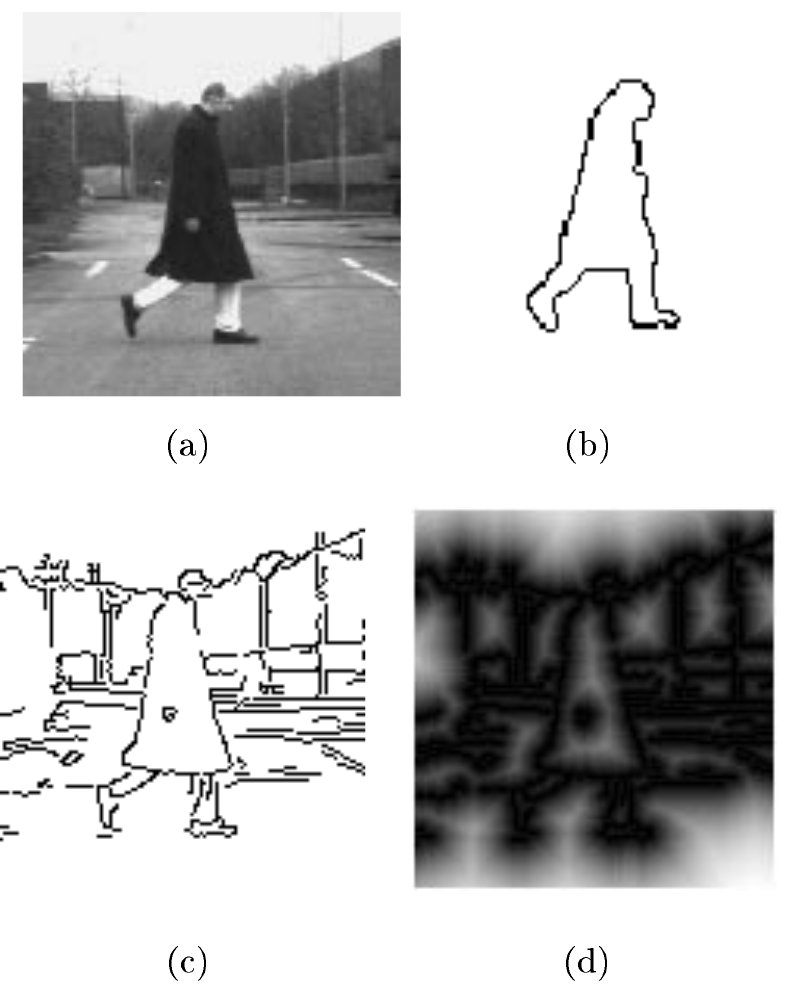
\includegraphics[width=0.65\linewidth]{pedestrian_detection.jpg}
\caption{a) původní obraz b) vzor c) nalezené hrany d) vyobrazené vzdálenosti
Převzato ~\cite{7} }
\label{pic3}
\end{figure}
\newpage 
%tady je "tato metoda" místo chemfer matching system
V rámci optimalizace se tato metoda rozšiřuje na hierarchizovanou, která sdružuje podobné vzory do shluků, a tudíž se prohledávání databáze zrychlí (viz obrázek~\ref{pic4}).
\begin{figure}[h]
\centering
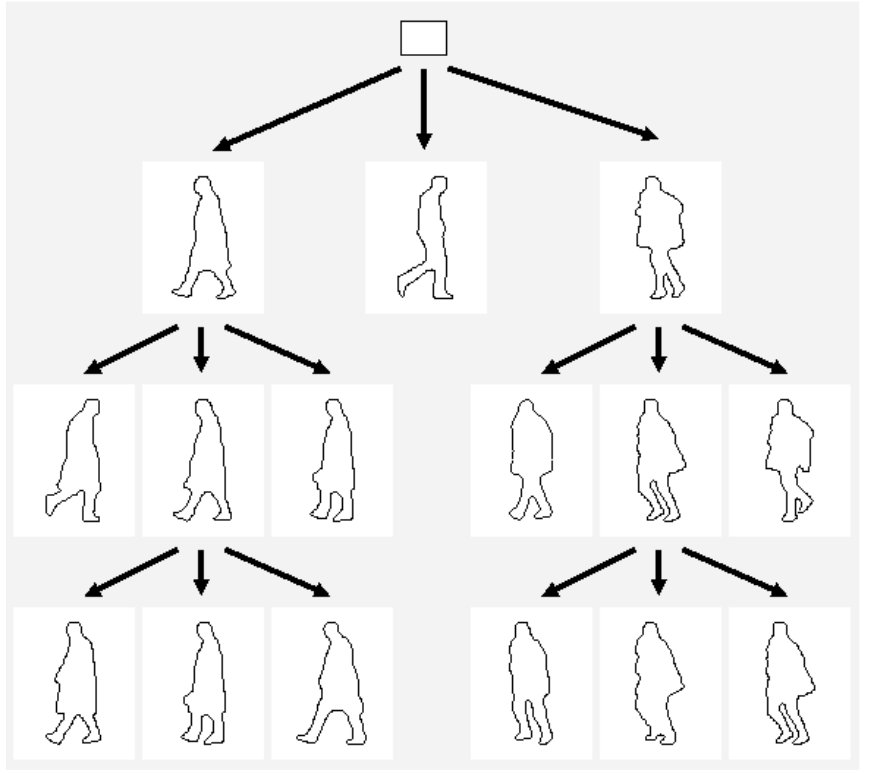
\includegraphics[width=0.6\linewidth]{hier.jpg}
\caption{Využití hierarchie v databázi vzorů. Převzato z ~\cite{7} }
\label{pic4}
\end{figure}

Ověření výsledku probíhá pomocí RBF klasifikátorem (neuronová síť založená na radiálních bázových funkcích). Nejdříve se z původního obrazu vybere čtyřúhelník obsahující možnou postavu a na základě euklidovské vzdálenosti se určuje, jestli jsou  jednotlivé pixely součástí postavy či nikoliv.\\
%RBF classifier!

Riggol a spol.~\cite{11} kombinují rozpoznávací metody založené na prvcích a na modelech za cílem dosažení spolehlivého a efektivního programu. Využívají P2DHMM (Pseudo-2D Hidden Markov Model). Jedná se o předem naučený algoritmus, který dokáže na základě pravděpodobností určit, jestli se jedná o postavu nebo ne. Příklad detekované postavy a postupné rozhodování je vidět na obrázku~\ref{pic5}.\\
\begin{figure}[h]
\centering
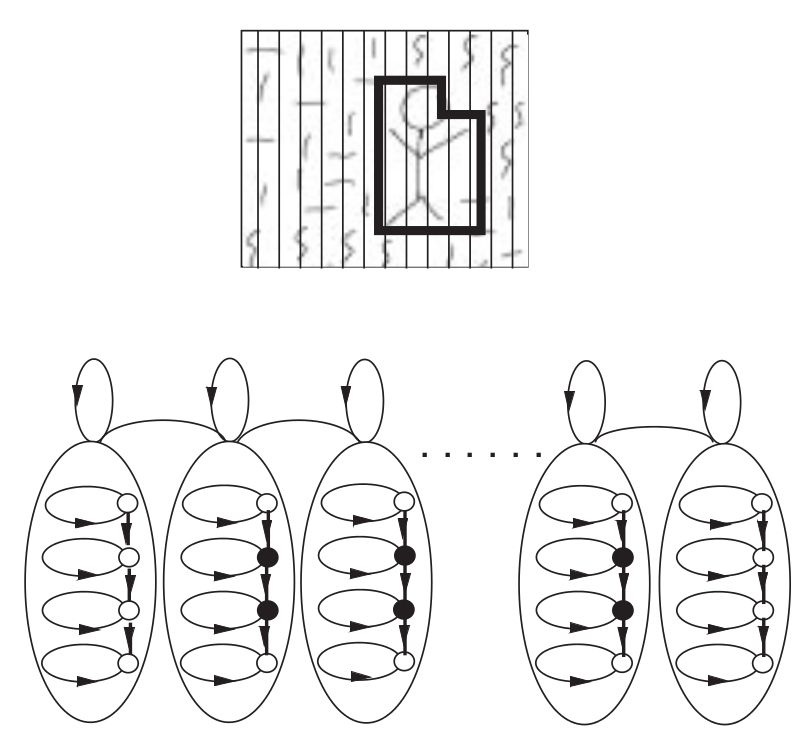
\includegraphics[width=0.5\linewidth]{P2DHMM.jpg}
\caption{Stochastický model 2D objektu s šumem okolo. Převzato z~\cite{11}. } %stochastic model of 2D object using P2DHMM
\label{pic5}
\end{figure}

\subsection{Rozpoznávání částí těla}
Ruka po zápěstí má 23 stupňů volnosti a v kombinaci s různým osvětlením a změnami v pozadí, se jedná o značně komplikovaný problém na řešení pomocí podobnosti.\\

Jestliže aplikace nevyžaduje přizpůsobení okolí (pozadí obrazu) a zůstává na stejném místě, lze použít rozdíl mezi objektem a pozadím~\cite{14}. To vyžaduje co nejvíce neměnné pozadí a dostatečný rozdíl mezi objektem a zbytkem. Rozdíl lze hledat jednoduše procházením pole nebo využitím 'chytrého' algoritmu, který spočívá v identifikaci části obrazu, která se pohybuje oproti posledním obrazům. Příklad detekce ruky odstraněním pozadí je ukázán na obrázku~\ref{pic6}. Pro účely bakalářské práce je metoda nevhodná, jelikož je potřeba řídit robota, který následuje člověka a tudíž nelze spoléhat na stejné okolí.

\begin{figure}[h]
\centering
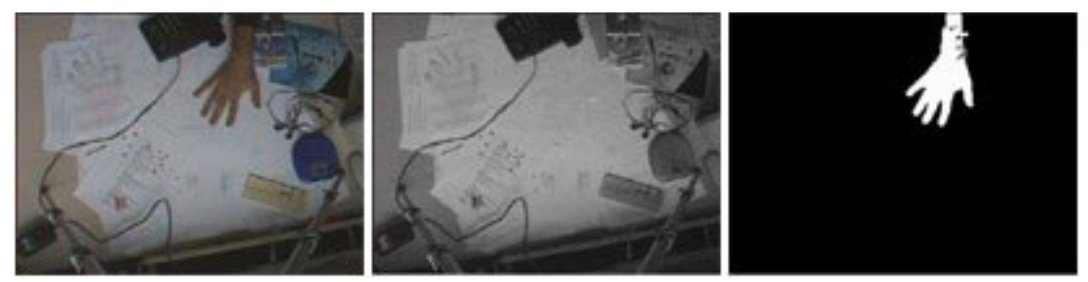
\includegraphics[width=1\linewidth]{diff.jpg}
\caption{a) vstup  b) referenční obraz  c) výstup 
(Převzato z~\cite{14}.) } 
\label{pic6}
\end{figure}


\subsection{Rozpoznávání gest}
Mezi rozpoznávání na základě vzhledu se řadí mnoho metod zahrnujících strojově naučené algoritmy jako neuronové sítě, HMM (Skrytý Markovův model) a jiné~\cite{3}. Gesto lze identifikovat i určením pozice a směru ruky a jednotlivých prstů.\\ %vyčetení/ identifikace?

Kim a spol.~\cite{5} používají bílé značky na špičkách prstů, které sledují černým světlem a detekují jednoznačně špičky prstů, což umožňuje velkou škálu možných gest. Na druhou stranu vzniká i omezení barvy pozadí, které lze eliminovat jen v určitém prostředí, tudíž se jedná o vhodnou variantu k využití například při hrách ve VR (virtuální realitě).\\

Shaker a Zliekha~\cite{12} získávají směr prstu ruky, kterou snímají dvě kamery. Jedna kamera natáčí shora zatímco druhá zboku. Gesto se rozpoznává z každého vstupu zvlášť. Nejdříve přepočítají obraz na stupně šedi a poté dle určené prahové hodnoty odfiltrují pozadí a vytvoří binární obraz. V tomto kroce je třeba, aby bylo pozadí jednoduché a jasně rozlišitelné od ruky. Kvůli odstranění šumu se obrázek rozmaže a následně zaostří. Je důležité, aby byla ruka největší objekt v obraze. Poté se pomocí Laplaciánovu operátoru získají hrany daného objektu a z nich se vytvoří kontury.
Gesto se identifikuje nalezením největšího vrcholu v obraze a nalezením hrany, kterou opisuje natažený prst a následnou kombinací obou směrů do 3D. Postup je znázorněný na obrázku~\ref{pic7}.

\begin{figure}[h]
\centering
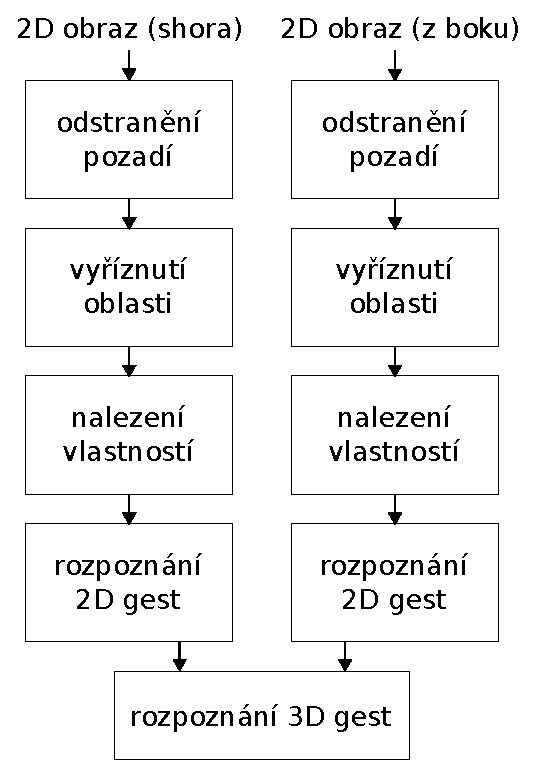
\includegraphics[width=0.4\linewidth]{pic7.eps}
\caption{Popis algoritmu dle Shakera a Zliekha. Přeloženo a převzato z~\cite{12}. } 
\label{pic7}
\end{figure}

\subsubsection{Rozpoznávání prstů}
Hackenberg a spol.~\cite{12} implementovali identifikaci prstů a dlaně na základě několika kroků. Nejprve projde hloubkový obraz z kamery a hledá tvary podobné špičkám prstů nebo rourovitého tvaru podobného prstům. Poté se zaměří na detailnější vlastnosti dlaně. Z nalezených vhodných polí, která mohou představovat dlaně se vyřadí ta, která nejsou napojena na prsty, nebo jsou menší než předem určená hodnota (odvozená od průměrně velikosti hlavy) a vzdáleností špiček prstů od dlaně.\\


Bez potřeby porovnávání tvarů a zdrojů se dají rozpoznat jednotlivé špičky prstů nalezením lokálního maxima v obrysu ruky. Ve všech adekvátních směrech se naleznou kandidáti a následně vyloučí mylné identifikace. Jedná se o postup náchylný na šum v obraze, podobná odolnější metoda navrhuje porovnávání vzdálenosti obrysu k pozici ruky~\cite{3}.\\
Jednotlivé prsty lze rozpoznat například pomocí vyhledávání na základě tvaru~\cite{4}. Jde o zjednodušení představy objektu na geometrický objekt a vyhledávání vhodných kandidátů v obraze, které mají tyčovitý tvar a délku v definovaných mezích. 

Mezi další programy rozpoznávající špičky prstů z již relativně čistého čtyřúhelníku, který obsahuje zájmový objekt, patří identifikace na základě dvou specifických vlastností. Střed špičky prstu je obklopen pixely patřící prstu a ty jsou obklopeny dlouhou řadou pixelů nepatřících prstu~\cite{14}. Ruce lze identifikovat i po nalezení prstů tím, že se vyloučí objekty podobného tvaru (propisky, fixy), které nesplňují vlastnosti rukou, například nejsou napojeny na žádnou dlaň. Nutná podmínka může být definována jako velikost úhlů mezi prsty. Vzdálenosti pixelů (bodů na ruce) lze počítat dle obrázku~\ref{pic8} pomocí vzorců: 

\begin{figure}[h]
\centering
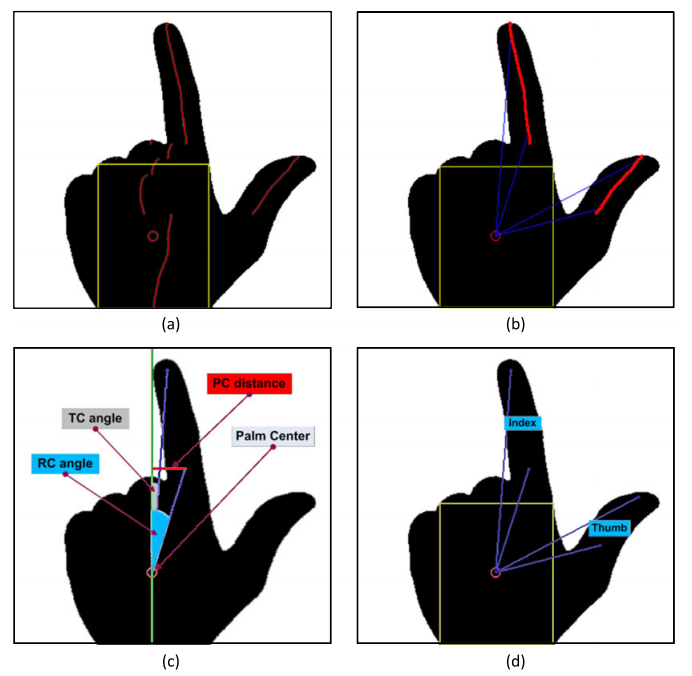
\includegraphics[width=0.5\linewidth]{fingers.png}
\caption{Vyobrazení definovaných pojmů, které lze využít k výpočtům pozic, na základě proporcionálních vlastností prstů.
(Převzato z~\cite{13}.) }
\label{pic8}
\end{figure}

\begin{center}
$RC_{angle} = 90 - tan^{-1} \frac{y_{r}-y_{pc}}{x_{r} - x_{pc}}$, \\
$TC_{angle} = 90 - tan^{-1} \frac{y_{ft}-y_{pc}}{x_{ft} - x_{pc}}$, 
\end{center}
kde $ RC_{angle} $ je úhel mezi přímkou vedenou vertikálně středem dlaně a spojnicí se středem počátku prstu, $ TC_{angle} $ je úhel mezi přímkou vedenou vertikálně středem dlaně a spojinicí se špičkou prstu, $ x_{pc}, y_{pc} $ souřadnice středu dlaně, $ x_{r}, y_{r} $ souřadnice středu počátku prstu a $ x_{ft}, y_{ft} $ souřadnice špičky prstu.

\newpage
\section{Aktuální aplikace rozpoznávání pomocí kamery}
\subsection{Možnosti využití gest při ovládání mobilního robotu}
Všechny aplikace, které mohou využít výhod~\cite{14} z práce:
\begin{itemize}
\item Ovládání elektronických zařízení na velmi malém prostoru
\item Ovládání elektronických zařízení z větší vzdálenosti
\item Snížený počet součástek (nejsou potřeba klávesnice a myš)
\item Zjednodušené ovládání elektroniky
\item Potenciál zabezpečení proti zneužití (při implementaci ochranných prvků)
\item Minimalistické (méně tlačítek a obdobných prvků)\\
\end{itemize}
Potenciál pro využití:
\begin{itemize}
\item Překlad znakové řeči
\item Ovládání chytrých zařízení (chytrá domácnost - světla, hudba, televize, telefon)
\item Prezentace před publikem (ovládání počítače)
\\
\end{itemize}
Již využíváno:
\begin{itemize}
\item Rozpoznání chodce v dohledu vozidla
\item Sociální experimenty (vyslání robotu stopovat)
\item Ovládání a hraní na konzolích
\end{itemize}

\subsection{Konkrétní aplikace používající Kinect nebo rozpoznávání gesta}
\subsubsection{Rehabilitace}
Mezi využítí kamery a rozpoznávání gest v lékařské oblasti patří převážně rehabilitační cvičení. V nemocnici ve městě Reading využívají kameru Kinect pacienti po mrtvici na zlepšení pohyblivosti a koordinace~\cite{21}. 

\subsubsection{Využití ve zdravotnictví}
Kinect lze dobře využít jako uživatelské rozhraní během operace, když chce doktor přístup k záznamům pacienta a nemusí se tak dotýkat žádných nesterilních věcí ~\cite{24}.\\

\subsubsection{Sport}
Kamera Kinect se využila i v experimentu provedeném na univerzitě v Sarawaku~\cite{22}. Cílem experimentu bylo nalezení vztahu mezi tepem a pohyby hráče badmintonu. Kamera snímala hráče při hře a měřila preciznost jednotlivých úderů. Výsledkem bylo, že při zvýšeném tepu klesá podávaný výkon, a tudíž lze lépe zamezit omdlévání při přetížení sportovců.

\subsubsection{Ovladač Bixi}
Bixi je bezdotykový ovladač k mobilnímu zařízení. Hlavním zaměřením je usnadnění ovládání vedlejších aplikací během řízení auta tak, aby se řidič mohl soustředit na provoz. Po spárování se zařízením přes bluetooth lze gesty volit adresu pro navigaci, ztišit či zastavit hudbu, ztlumit jas obrazovky, přijímat hovory a jiné~\cite{bixi}.

\subsubsection{DJI drony}
Drony od společnosti Da-Jiang Innovations~\cite{dji} již také využívají rozpoznávání gest k ovládání. Mavic, Phanton 4 Pro, Advance  a Spark podporují focení, které se zapne vykreslením žádaného rámečku fotky rukou.

Spark podporuje mnohem více funkcí ovládaných gesty. Po natažení ruky směrem dopředu a nahoru k dronu pod úhlem $ 45^\circ $ se začne nahrávat video. Podporuje také vznášení se z dlaně a přistávání na dlaň. Pro vzlet je třeba držet dron na dlaně kamerou k obličeji, aby ho to rozpoznalo, a následně se vznese. Po mávnutí rukou před kamerou jedním ze čtyř hlavních směrů se dron posune daným směrem. Při zamávání začne dron následovat trajektorii chůze člověka. Při detekci dlaně pod sebou na ni dron přistane~\cite{heliguy}.

\endinput
%%
%% End of file `ch01.tex'.
